
\section{UART and I2C}

\subsection{UART - Universal Asynchronous Receiver Transmitter}

\mult{2}

\begin{definition}{UART}\\ is an asynchronous serial communication interface:
    \vspace{1mm}\\
    \textbf{Asynchronous data transfer}
    \begin{itemize}
        \item Mismatch of clock frequencies in TX and RX $\rightarrow$ no shared clock between transmitter and receiver
        \item Overhead for synchronization $\rightarrow$ extra Bits
        \item Effort for synchronization $\rightarrow$ extra Hardware
    \end{itemize}
    \vspace{1mm}

    \textbf{Full-duplex communication}
    \begin{itemize}
        \item Point-to-point communication (one transmitter, one receiver)
        \item Full-duplex (simultaneous bidirectional communication)
        \item Start and stop bits used for synchronization
        \item Typically 2-wire interface (TX and RX) for data
        \item Optional control signals (RTS/CTS, etc.) for flow control
    \end{itemize}

    \textbf{Advantages}
    \begin{itemize}
        \item Clock does not have to be transmitted
        \item transmission delays automatically compensated
        \item no need for a common clock signal
    \end{itemize}
    \vspace{1mm}
    
    \textbf{Disadvantages}
    \begin{itemize}
        \item Synchronization at start of each data item
        \item Limited to point-to-point communication
        \item Slower than synchronous protocols (e.g., SPI)
        \item More complex error handling due to asynchronous nature
    \end{itemize}
\end{definition}

\begin{concept}{UART Synchronization}
\begin{itemize}
    \item Receiver \textbf{detects start bit} \\ (falling edge from idle to '0')
    \item Receiver \textbf{samples} middle of each bit based on configured baud rate
    \item Both devices must use the same \textbf{configuration}:
    \begin{itemize}
        \item Baud rate (e.g., 9600, 115200 bits/s)
        \item Number of data bits (5-8)
        \item Parity (none, odd, even, mark, space)
        \item Number of stop bits (1, 1.5, 2)
    \end{itemize}
\end{itemize}
\end{concept}

\begin{concept}{UART Transmission}\\
    Connecting shift registers with diverging clock sources:
    \begin{itemize}
        \item same target frequency
        \item different tolerances and divider ratios
        \item requires \textbf{synchronization} at start of each data item receiver \\ $\rightarrow$ each data item (5-8 bits) req. synchron.
    \end{itemize}
    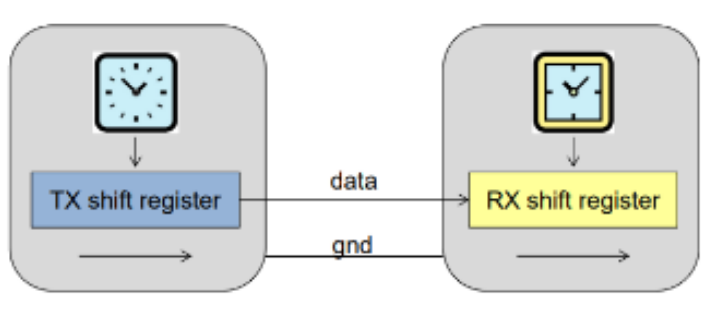
\includegraphics[width=\linewidth]{uart.png}
    
    \textbf{On-Board Connections}
    \begin{itemize}
        \item Signal Levels: 3V or 5V with reference to ground
        \item Off-Board connections req. strong output drivers 
    \end{itemize}
\end{concept}

\begin{theorem}{UART Signals}
Basic UART connections require:\\
\textbf{TX} (Transmit): \small{Data output (transmitter to receiver)}\\
\normalsize
\textbf{RX} (Receive): Data input (transmitter to receiver)\\
\textbf{GND} (Ground): Common reference level
\vspace{1mm}\\
\textcolor{frog}{\textbf{Extended UART}} (with hardware flow control):
\begin{itemize}
    \item \textbf{RTS} (Request to Send): Output indicating readiness to send
    \item \textbf{CTS} (Clear to Send): Input indicating partner is ready to receive
\end{itemize}
\end{theorem}

\begin{corollary}{UART Frame Structure}
\begin{itemize}
    \item \textbf{Idle state}: Line is high ('1') when no transmission occurs
    \item \textbf{Start bit}: Always '0', signals beginning of frame
    \item \textbf{Data bits}: 5 to 9 bits (typically 8), LSB first
    \item \textbf{Parity bit} (optional): For error detection
    \item \textbf{Stop bit(s)}: 1, 1.5, or 2 bits, always '1'
\end{itemize}
\end{corollary}

\multend

\subsection{UART Timing and Calculations}

\mult{2}

\begin{formula}{UART Calculations}
\vspace{1mm}\\
\textbf{Bit Time (seconds):}
$\quad T_{bit} = \frac{1}{\text{Baud Rate}}$
\vspace{2mm}\\
\textbf{Frame Time (seconds):}
$$T_{frame} = T_{bit} \times \text{Total Bits per Frame (TBF)}$$
\small{TBF = 1 (start) + Data Bits + Parity Bits + Stop Bits}
\vspace{2mm}\\
\normalsize
\textbf{Maximum Data Rate (bytes/second):}
$$\text{Data Rate} = \frac{\text{Baud Rate}}{\text{Total Bits per Byte (TBB)}}$$
\small{TBB = 1 (start) + Data Bits + Parity Bits + Stop Bits}
\end{formula}

\begin{KR}{Clock Tolerance in UART}\\
\textbf{Maximum clock deviation}:
The receiver must sample correctly until last bit!

Maximum allowed clock deviation (as percentage):
$$\text{Deviation}_{\max} = \frac{0.5}{N} \times 100\%$$

\small {N = number of bit times between synchronization points}
\end{KR}

\begin{example}
    For a standard UART frame (1 start, 8 data, 1 stop):\\
    Synchronization at start bit,
    Last bit (stop bit) 10 bits later
    \vspace{1mm}\\
    Maximum clock deviation = 0.5/10 = 5\%\\
    Sample calculation:
    If sender clock 9600 Hz: Receiver between 9120 Hz and 10080 Hz
\end{example}

\multend

\begin{KR}{Analyzing UART Transmission}


\paragraph{Identify frame/bit structure}
\begin{itemize}
    \item Start bit: Always '0' (falling edge)
    \item Data bits: LSB first, 5-8 bits
    \item Parity bit: Optional, can be even, odd, mark ('1'), or space ('0')
    \item Stop bit(s): Always '1' (can be 1, 1.5, or 2 bits)
    \item Idle state: Line remains high ('1') $\rightarrow$ no transmission
\end{itemize}
Receiver synchronizes anew at each start bit.

\paragraph{Calculations}
\begin{itemize}
    \item See formulas \textcolor{purple}{\textbf{UART Calculations}} and \textcolor{pink}{\textbf{Clock Tolerance in UART}}
    \item Clock Tolerance/Taktabweichung: max. deviation = 0.5T (Bit-Zeit) at last data bit (sync. only at start bit)
\end{itemize}

\paragraph{Timing diagram}
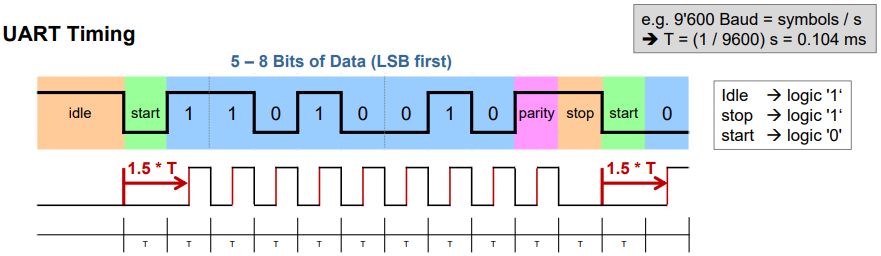
\includegraphics[width=0.8\linewidth]{uart_tiiming_diagram_overview.png}
\end{KR}

\begin{example2}{UART Übertragung 'AC'}
    UART mit 19200 Bit/s, 7 Daten-Bits, 1 Stop-Bit (kein Parity)

    ASCII('A') = 0x41 = 100 0001b, ASCII('C') = 0x43 = 100 0011b
    
    \tcblower
    \textbf{Calculations:}
    \begin{itemize}
        \item Bit-Zeit: T = 1/19200 s = 52.1 $\mu$s
        \item Total Bits per Frame (TBF) = 1S (start) + 7D (data) + 1E (stop) = 9 Bits $\rightarrow$ for each frame/character
        \item Frame Time: $T_{frame}$ = TBF $\times$ T = 9 Bits $\times$ 52.1 $\mu$s = 469.0 $\mu$s $\rightarrow$ for each frame/character
        \item Total Transmission Time: $2 \times T_{frame} = 938.0 \mu s$
    \end{itemize}
    Between frames, the line is idle (I) - high.
    \vspace{1mm}\\
    \textbf{Timing Diagram:}
    \vspace{1mm}\\
    \begin{minipage}{0.5\linewidth}
    Frame for 'A' (0x41 = 100 0001b):
    \begin{itemize}
        \item Start bit (S): 0
        \item Data bits (D), LSB first: 1, 0, 0, 0, 0, 0, 1
        \item Stop bit (E): 1
    \end{itemize}
    \end{minipage}
    \begin{minipage}{0.5\linewidth}
    Frame for 'C' (0x43 = 100 0011b):
    \begin{itemize}
        \item Start bit (S): 0
        \item Data bits (D), LSB first: 1, 1, 0, 0, 0, 0, 1
        \item Stop bit (E): 1
    \end{itemize}
    \end{minipage}
    \vspace{1mm}\\
    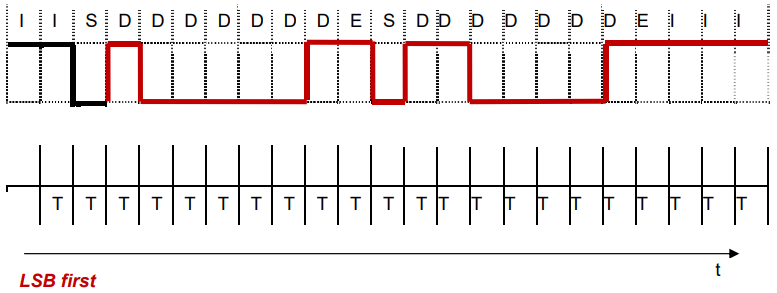
\includegraphics[width=0.7\linewidth]{uart_timing_ex.png}
    
    \textbf{Legende:}
    \begin{itemize}
        \item I = Idle-Bit, S = Start-Bit, D = Daten-Bit, E = Stop-Bit
        \item LSB first: Daten-Bits werden von rechts nach links übertragen
    \end{itemize}
    
    \textbf{Taktabweichung (Clock Deviation):}
    \begin{itemize}
        \item Fallende Flanke Start-Bit bis Mitte D6 = 7.5 Bits
        \item Max. Abweichung für D6: 0.5 Bits
        \item Taktabweichung: 100\% $\times$ 0.5 / 7.5 = 6.67\%
        \item Bei 19200 Bit/s: 19200 $\times$ 6.67\% = 1280 Bit/s \\ $\Rightarrow$ Empfänger-Takt (Receiver Clock) zwischen 17920 Bit/s und 20480 Bit/s
    \end{itemize}
\end{example2}

\subsection{UART Implementation}

\begin{definition}{Implementation of UART with Shift Registers}
    Example: 9600 Baud with selected quartz frequencies

    \begin{minipage}{0.7\linewidth}
    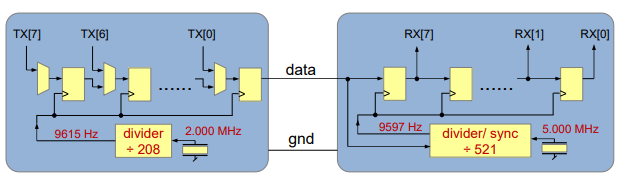
\includegraphics[width= \linewidth]{uart_implementation_shift.png}
    \end{minipage}
    \begin{minipage}{0.3\linewidth}
    Transmission and receiver use closest integer to divide clock:
    \begin{itemize}
        \item 2000/208 = 9615 Hz \\ $\rightarrow$ Slightly too fast
        \item 5000/521 = 9597 Hz \\ $\rightarrow$ Slightly too slow
    \end{itemize}
    $\rightarrow$ Settings allow \\ successful transmission
    \end{minipage}
\end{definition}

\begin{concept}{STM32F4 UART/USART Peripherals}
The STM32F4 includes several UART/USART modules with:

\begin{minipage}{0.5\linewidth}
\begin{itemize}
    \item Full-duplex communication (USART)
    \item Programmable baud rate
    \item Interrupt generation on events \\ (TX empty, RX not empty, etc.)
    \end{itemize}
\end{minipage}
\begin{minipage}{0.5\linewidth}
\begin{itemize}
    \item Configurable data bits, stop bits, and parity
    \item DMA support for efficient data transfer
    \item Hardware flow control (CTS/RTS) on USARTs
    \item Synchronous mode available on USARTs
\end{itemize}
\end{minipage}
\end{concept}

\begin{code}{STM32F4 UART Configuration} Configure UART2 for 115200 baud, 8-N-1
\begin{lstlisting}[language=C, style=basesmol]
// 1. Enable UART2 and GPIO clock
RCC->APB1ENR |= RCC_APB1ENR_USART2EN;  // Enable UART2 clock
RCC->AHB1ENR |= RCC_AHB1ENR_GPIOAEN;   // Enable GPIOA clock
// 2. Configure GPIO pins for UART (PA2 = TX, PA3 = RX)
// Set alternate function mode (0x10)
GPIOA->MODER &= ~(0x3 << (2*2) | 0x3 << (2*3));
GPIOA->MODER |= (0x2 << (2*2) | 0x2 << (2*3));
// Set to AF7 (UART2)
GPIOA->AFR[0] &= ~(0xF << (4*2) | 0xF << (4*3));
GPIOA->AFR[0] |= (0x7 << (4*2) | 0x7 << (4*3));
// 3. Configure UART
// Reset UART configuration
USART2->CR1 = 0;
USART2->CR2 = 0;
USART2->CR3 = 0;
// Set baud rate (assuming 84MHz APB1 clock)
// BRR = f_CK / baud rate = 84,000,000 / 115,200 = 729.16
USART2->BRR = 729;
// Enable UART, TX, and RX
USART2->CR1 = USART_CR1_UE | USART_CR1_TE | USART_CR1_RE;
\end{lstlisting}
\end{code}

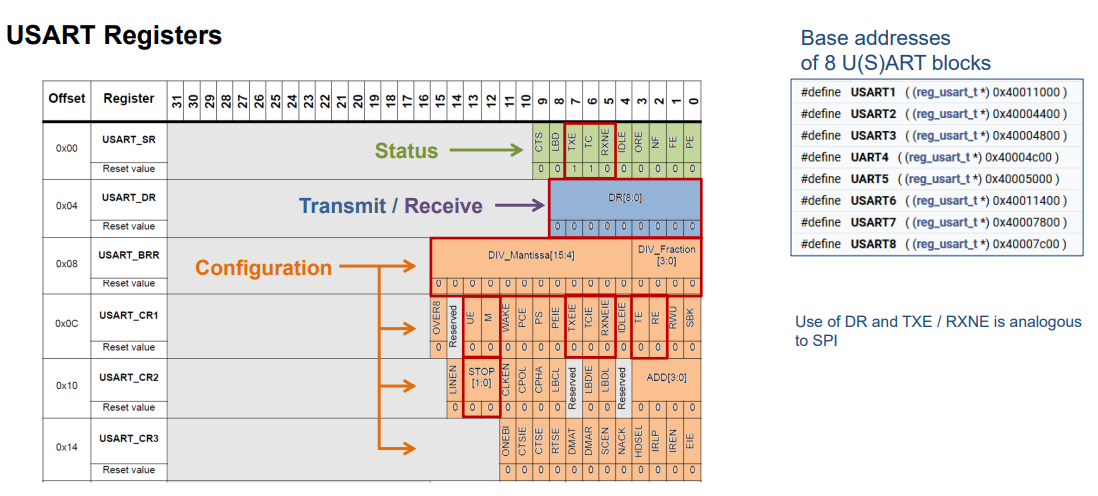
\includegraphics[width=\linewidth]{uart_registers.png}

\begin{KR}{UART Data Transmission and Reception}\\
\textbf{Transmitting Data}
Write data to the data register after checking the TXE flag.\\
\textbf{Receiving Data}
Read from the data register after checking the RXNE flag.

\begin{lstlisting}[language=C, style=basesmol]
// Send a character
void UART_SendChar(USART_TypeDef *uart, char c) {
    // Wait until TXE flag is set (transmit buffer empty)
    while (!(uart->SR & USART_SR_TXE)) { }
    // Write the character to the data register
    uart->DR = c;
}
// Send a string
void UART_SendString(USART_TypeDef *uart, const char *str) {
    while (*str) {
        UART_SendChar(uart, *str++);
    }
}
// Receive a character (blocking)
char UART_ReceiveChar(USART_TypeDef *uart) {
    // Wait until RXNE flag is set (data received)
    while (!(uart->SR & USART_SR_RXNE)) { }
    // Return received data
    return uart->DR;
}
\end{lstlisting}
\end{KR}

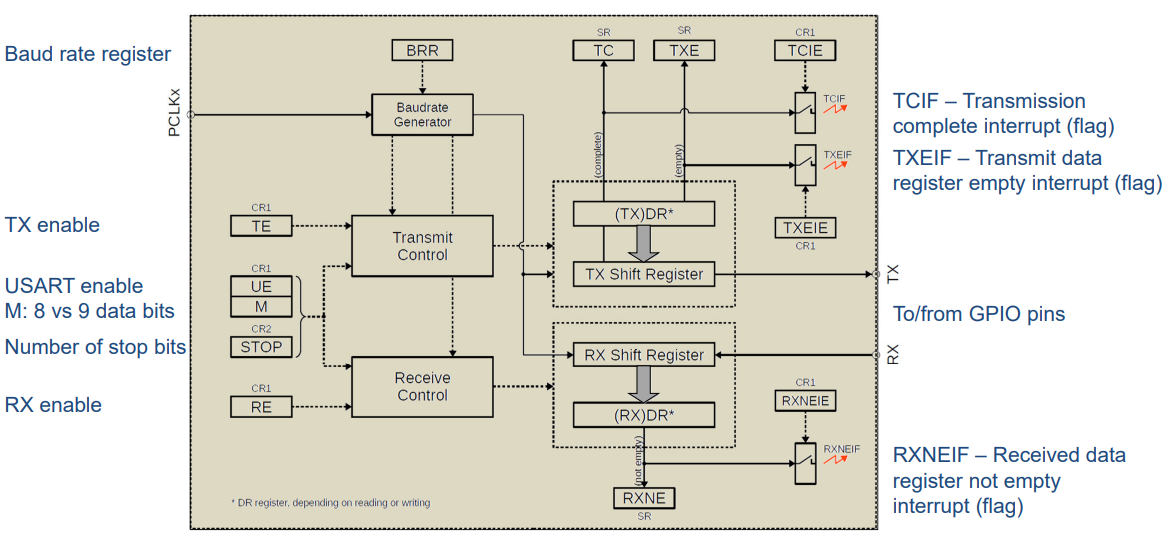
\includegraphics[width=\linewidth]{uart_on_stm.png}




\raggedcolumns
\columnbreak
\subsubsection{Electrical Characteristics of UART}

\begin{definition}{RS232 - Interconnecting Equipment by Cable}

    \begin{minipage}{0.7\linewidth}
        \begin{itemize}
            \item Simple, bidirectional point-to-point interface based on UART
            \item Optional control signals, e.g. CTS - Clear To Send
            \item Ground $\rightarrow$ common reference level for all signals (single ended)
            \item Driver circuit allows transmissions up to $\sim 10 \mathrm{~m}$
            \item Logic '1' -3V to -15V and Logic '0' 3 V to 15 V
        \end{itemize}
    \end{minipage}
    \begin{minipage}{0.3\linewidth}
    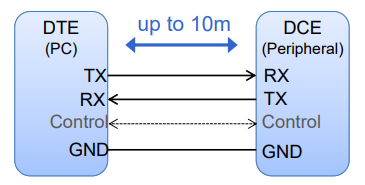
\includegraphics[width=\linewidth]{uart_cable.png}
    \end{minipage}
    
\end{definition}



\begin{concept}{RS232 - Interconnecting Equipment by Cable}
    RS-485 - Differential Transmission Based on UART
    \begin{itemize}
        \item Differential signals 
        \item Less susceptible to disturbances $\rightarrow$ longer distances, 100+ Meters
        \item Transmit and receive share the same lines
        \item Industrial automation: lowest layer of Profibus
    \end{itemize}
    \begin{center}
    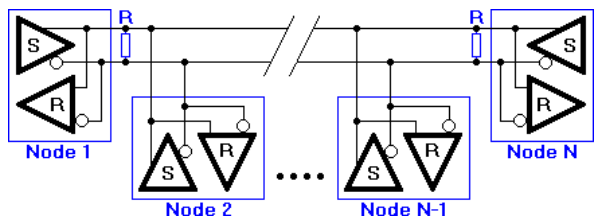
\includegraphics[width=0.6\linewidth]{uart_interconnection1.png}
    \end{center}
\end{concept}

\begin{theorem}
    {RS-485 - Differential Transmission}
    \begin{itemize}
        \item Transmitter transforms single-ended signal into differential signal
        \item Capacitive coupled noise affects both lines
        \item Receiver forms the difference of the two signals
        \item Noise on the two lines cancels itself to a large extent
    \end{itemize}
    \begin{center}
    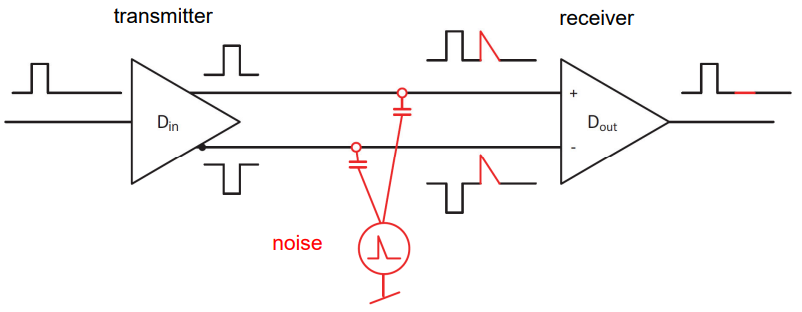
\includegraphics[width=0.7\linewidth]{uart_interconnection2.png}
    \end{center}
\end{theorem}


\raggedcolumns
\pagebreak






\subsection{I2C - Inter-Integrated Circuit}




\begin{definition}{I2C} synchronous, half-duplex, multi-master bus:

\begin{minipage}{0.5\linewidth}
\begin{itemize}
    \item 2-wire interface (SCL=Clock and SDA=Data)
    \item Multi-master, multi-slave capability
    \item Unique 7-bit or 10-bit address for each device
    \item Synchronous (master provides clock)
\end{itemize}
\end{minipage}
\begin{minipage}{0.5\linewidth}
\begin{itemize}
    \item Half-duplex (data flows in one direction at a time)
    \item 8-bit oriented data transfers
    \item Well-suited for connecting multiple boards or chips
    \item Bit rates from 100 kbit/s (standard) to 5 Mbit/s (ultra-fast)
\end{itemize}
\end{minipage}

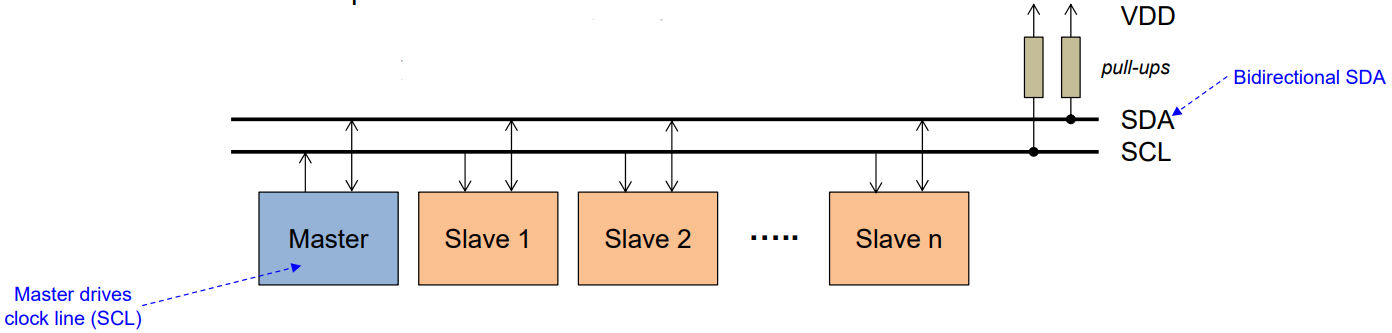
\includegraphics[width=0.8\linewidth]{i2c_bus.png}
\end{definition}

\mult{2}

\begin{concept}{Driving Data on SDA}\\
    Data driven onto SDA by master or addressed slave:
    \begin{itemize}
        \item depending on transaction (read/write) and point in time
        \item Change of data only allowed when SCL is low
        \item Allows detection of START and STOP conditions
    \end{itemize}
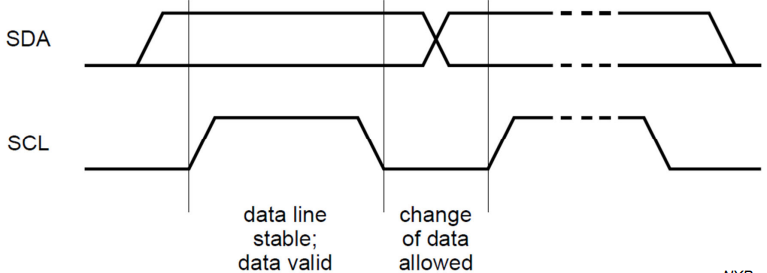
\includegraphics[width=\linewidth]{sda_data_lines.png}
I2C requires just two bidirectional lines (both open-drain) with external pull-up resistors:
\begin{itemize}
    \item \textbf{SCL} (Serial Clock Line): Clock signal generated by master
    \item \textbf{SDA} (Serial Data Line): Bidirectional data line
\end{itemize}
\end{concept}

\begin{theorem}{I2C Operation}
    \begin{itemize}
        \item Master drives clock line (SCL)
        \item Master initiates communication with START condition
        \item Master terminates
    \end{itemize}
    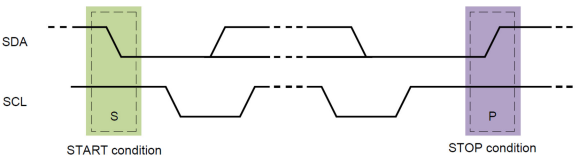
\includegraphics[width=\linewidth]{I2C_operation.png}
\end{theorem}

\begin{corollary}{I2C Bus Conditions}
\begin{itemize}
    \item \textbf{START condition}: SDA goes from high to low while SCL is high
    \item \textbf{STOP condition}: SDA goes from low to high while SCL is high
    \item \textbf{Data valid}: SDA remains stable while SCL is high
    \item \textbf{Data change}: SDA changes only when SCL is low
\end{itemize}
\end{corollary}

\multend

\begin{formula}{I2C Data Transfer}
Data transfer sequence: (8-bit oriented transfers, MSB first, receiver acknowledges each byte)
\begin{itemize}
    \item Master initiates transfer with START condition
    \item Master sends 7-bit slave address + R/W bit (0 = write, 1 = read)
    \item Addressed slave acknowledges (ACK) by pulling SDA low
    \item Data bytes transferred (8 bits followed by ACK/NACK)
    \item Master terminates transfer with STOP condition (determines number of transfers)
\end{itemize}
Bit 9: Receiver acknowledges by pulling SDA low during 9th clock cycle (ACK) or remains high (NACK).
\vspace{1mm}\\
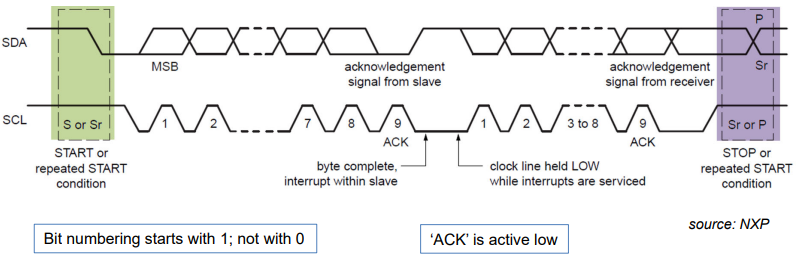
\includegraphics[width=\linewidth]{i2c_data_transfer.png}

\end{formula}



\begin{minipage}{0.6\linewidth}

\begin{concept}{I2C Accesses}\\
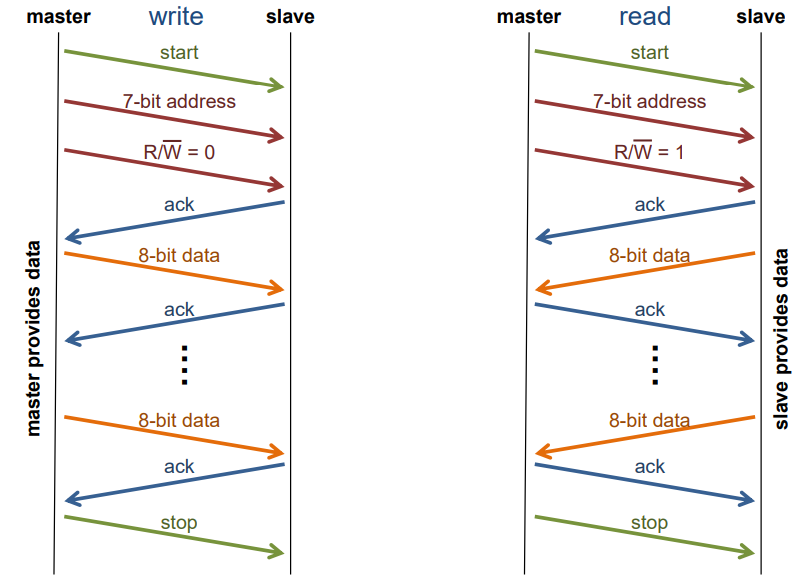
\includegraphics[width=\linewidth]{i2c_accesses.png}
\end{concept}
\end{minipage}
\begin{minipage}{0.4\linewidth}
\begin{corollary}{I2C Acknowledge and Not-Acknowledge}\\
After each byte transfer:
\begin{itemize}
    \item \textbf{ACK} (Acknowledge): Receiver pulls SDA low during 9th clock cycle
    \item \textbf{NACK} (Not-Acknowledge): SDA remains high during 9th clock cycle
\end{itemize}
\vspace{1mm}
NACK can indicate:
\begin{itemize}
    \item No receiver with the transmitted address
    \item Receiver unable to receive or transmit
    \item Receiver doesn't understand the data/command
    \item Receiver cannot receive more data
    \item Master-receiver signals end of transfer to slave-transmitter
\end{itemize}
\end{corollary}
\end{minipage}



\mult{2}

\begin{example2}{I2C Write Operation}\\
Master wants to write data 0x9C to slave with address 0x66
\tcblower
\begin{enumerate}
    \item Master generates START condition
    \item Master sends slave address (0x66) with \\ R/W = 0 (write): 0xCC
    \item Slave acknowledges (ACK)
    \item Master sends data byte 0x9C
    \item Slave acknowledges (ACK)
    \item Master generates STOP condition
\end{enumerate}
I2C bus:\\
START - 0xCC - ACK - 0x9C - ACK - STOP
\end{example2}

\begin{example2}{I2C Read Operation}\\
Master wants to read data from slave with address 0x66
\tcblower
\begin{enumerate}
    \item Master generates START condition
    \item Master sends slave address (0x66) with \\ R/W = 1 (read): 0xCD
    \item Slave acknowledges (ACK)
    \item Slave sends data byte (e.g., 0x9C)
    \item Master sends NACK to indicate end of transfer
    \item Master generates STOP condition
\end{enumerate}
I2C bus:\\
START - 0xCD - ACK - 0x9C - NACK - STOP
\end{example2}

\multend

\subsubsection{I2C Timing and Protocol}

\begin{concept}{I2C Timing} MSB first!\\
    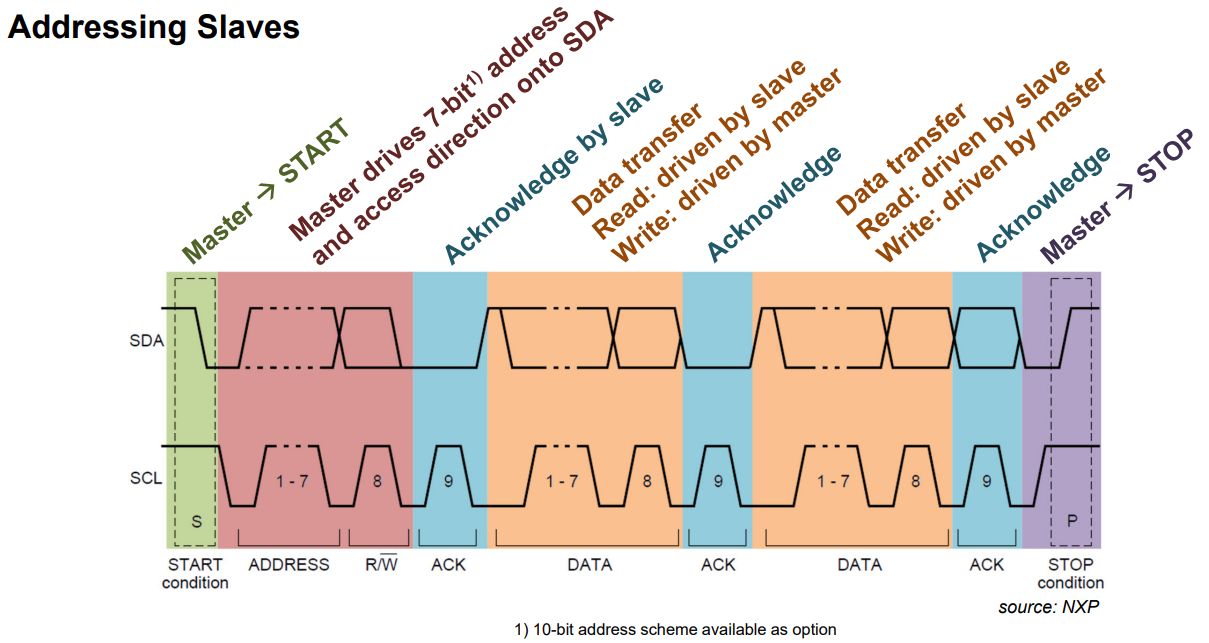
\includegraphics[width=0.9\linewidth]{i2c_timing_slave_addressing.png}\\
    ACK = 0 $\rightarrow$ Übertragung erfolgreich\\
    ACK = 1 $\rightarrow$ Übertragung nicht erfolgreich
\end{concept}




\begin{KR}{Analyzing I2C Communication}
\paragraph{Identify I2C protocol elements}
\begin{itemize}
    \item Start condition: SDA falls while SCL is high
    \item Stop condition: SDA rises while SCL is high
    \item Data bit transfer: SDA stable while SCL is high
    \item Acknowledge (ACK): Receiver pulls SDA low during 9th clock cycle
    \item Not-acknowledge (NACK): SDA remains high during 9th clock cycle
\end{itemize}

\paragraph{Parse I2C frames}
\begin{itemize}
    \item First byte after start: 7-bit address + R/W bit
    \begin{itemize}
        \item R/W = 0: Write operation
        \item R/W = 1: Read operation
    \end{itemize}
    \item Check for ACK/NACK after each byte
    \item Data bytes follow (8 bits each)
    \item Master or slave can end transmission with STOP condition
\end{itemize}

\paragraph{Interpret timing diagram}
\begin{itemize}
    \item Examine SCL and SDA lines
    \item Identify start and stop conditions
    \item Group bits into bytes (8 bits + ACK/NACK)
    \item Determine if each byte is address or data
    \item Note the direction of data transfer
\end{itemize}
\end{KR}

\begin{example2}{I2C Communication Analysis}\\
Analyze the following I2C timing diagram and describe the transaction: (ACK is active low)

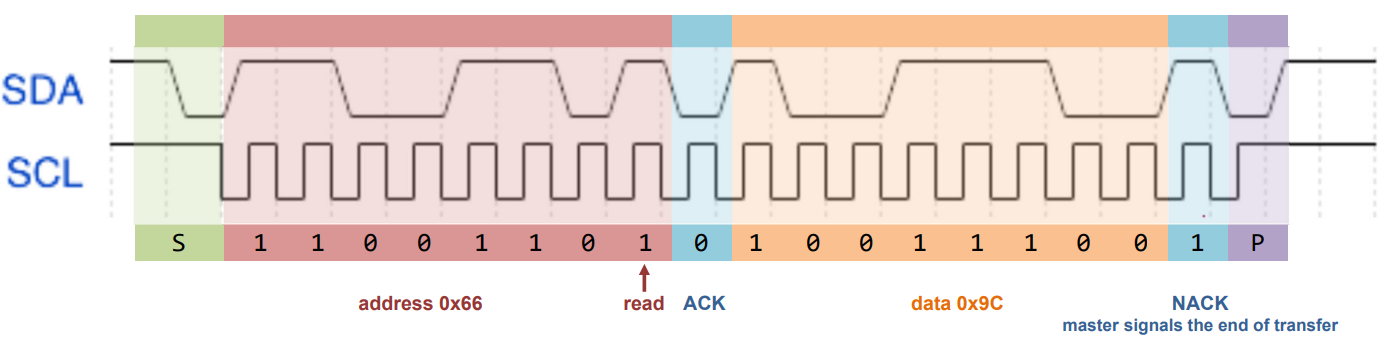
\includegraphics[width=\linewidth]{i2c_timing_example.png}

\tcblower
The I2C transaction consists of:
\begin{enumerate}
    \item Start condition (SDA falls while SCL is high)
    \item First byte: 11001101 (data transmitted MSB first)
    \begin{itemize}
        \item This is the address byte: 1100110 (0x66) with R/W bit = 1 (read operation)
        \item Followed by an ACK (SDA pulled low during 9th clock cycle)
    \end{itemize}
    \item Second byte: 00111001 (data received from slave)
    \begin{itemize}
        \item This is data: 0x39 or 0x9C (depending on bit order interpretation)
        \item Followed by a NACK (SDA remains high during 9th clock cycle)
        \item NACK indicates that the master does not want to receive more data
    \end{itemize}
    \item Stop condition (SDA rises while SCL is high)
\end{enumerate}
\vspace{1mm}
\textbf{The complete transaction is:}
\begin{itemize}
    \item Master initiates communication with device at address 0x66
    \item Master requests to read from the device (R/W=1)
    \item Device acknowledges (ACK)
    \item Device sends one data byte (0x39 or 0x9C)
    \item Master signals end of transfer with NACK
    \item Master terminates communication
\end{itemize}
\end{example2}


\raggedcolumns
\pagebreak

\subsubsection{I2C on STM32F4}

\begin{concept}{STM32F4 I2C Peripherals}\\
The STM32F4 includes I2C modules with features:
\vspace{2mm}\\
\begin{minipage}{0.5\linewidth}
\begin{itemize}
    \item Compatible with I2C standard protocol
    \item Multiple speed modes (standard, fast)
    \item 7-bit and 10-bit addressing
    \item Multi-master capability
    \end{itemize}
\end{minipage}
\begin{minipage}{0.5\linewidth}
\begin{itemize}
    \item Programmable clock stretching
    \item Programmable NOSTRETCH capability
    \item DMA support for efficient data transfer
    \item SMBus support
\end{itemize}
\end{minipage}
\end{concept}

\begin{code}{STM32F4 I2C Configuration}
\begin{lstlisting}[language=C, style=basesmol]
// Configure I2C1 for 100kHz standard mode
// 1. Enable I2C1 and GPIO clock
RCC->APB1ENR |= RCC_APB1ENR_I2C1EN;   // Enable I2C1 clock
RCC->AHB1ENR |= RCC_AHB1ENR_GPIOBEN;  // Enable GPIOB clock

// 2. Configure GPIO pins for I2C (PB6 = SCL, PB7 = SDA)
// Set alternate function mode (0x10)
GPIOB->MODER &= ~(0x3 << (2*6) | 0x3 << (2*7));
GPIOB->MODER |= (0x2 << (2*6) | 0x2 << (2*7));
// Set open-drain output type
GPIOB->OTYPER |= (1 << 6) | (1 << 7);
// Set to AF4 (I2C1)
GPIOB->AFR[0] &= ~(0xF << (4*6) | 0xF << (4*7));
GPIOB->AFR[0] |= (0x4 << (4*6) | 0x4 << (4*7));

// 3. Reset I2C
I2C1->CR1 = I2C_CR1_SWRST;  // Software reset
I2C1->CR1 = 0;              // Clear reset

// 4. Configure I2C
// Set peripheral clock frequency (42MHz)
I2C1->CR2 = 42;  // FREQ = 42MHz
// Set CCR for 100kHz standard mode
// CCR = PCLK1 / (2 * I2C_FREQ) = 42MHz / (2 * 100kHz) = 210
I2C1->CCR = 210;
// Set TRISE
// TRISE = (max rise time * PCLK1) + 1 = (1000ns * 42MHz) + 1 = 43
I2C1->TRISE = 43;
// 5. Enable I2C
I2C1->CR1 |= I2C_CR1_PE;  // Peripheral enable
\end{lstlisting}
\end{code}

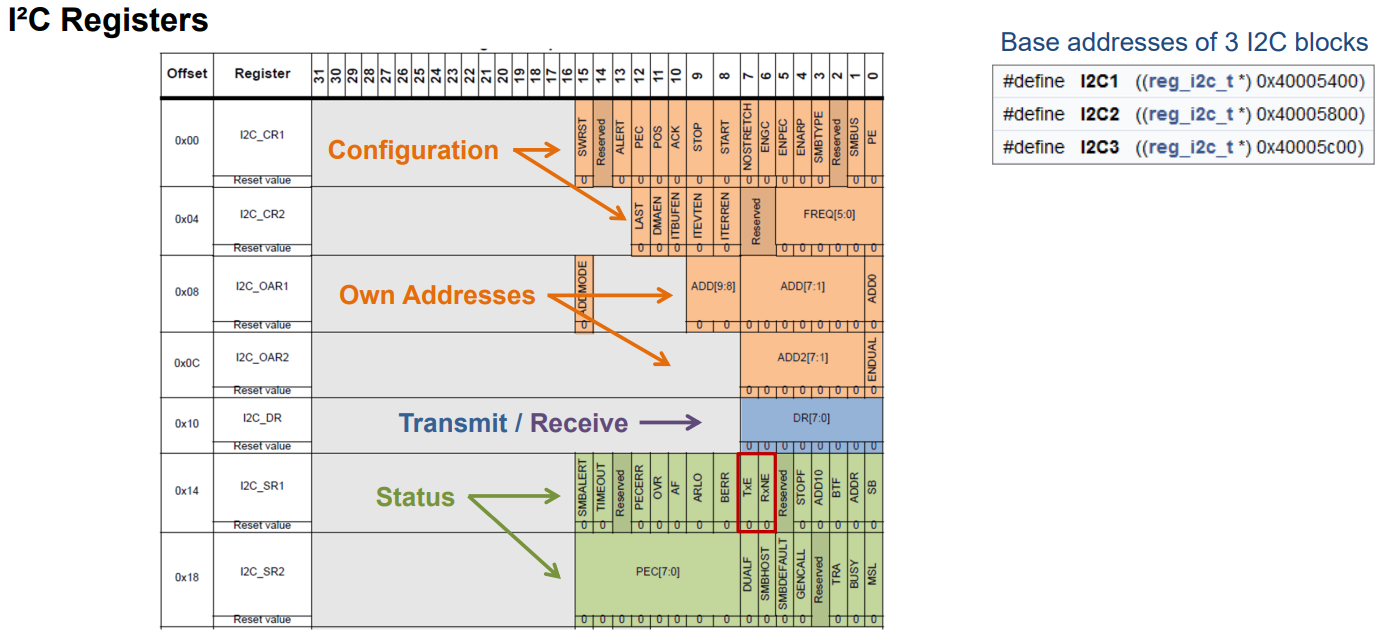
\includegraphics[width=\linewidth]{i2c_registers.png}

\begin{KR}{I2C Master Transmit and Receive}
\paragraph{Master Transmit Sequence}
Generate START, send address+write, send data bytes, generate STOP.
\paragraph{Master Receive Sequence}
Generate START, send address+read, receive data bytes with ACK/NACK, generate STOP.

\begin{lstlisting}[language=C, style=basesmol]
// I2C Master Transmit
void I2C_MasterTransmit(I2C_TypeDef *i2c, uint8_t address, uint8_t *data, uint16_t size) {
    // 1. Wait until I2C bus is free
    while (i2c->SR2 & I2C_SR2_BUSY) { }
    // 2. Generate START condition
    i2c->CR1 |= I2C_CR1_START;
    // 3. Wait for EV5 (START sent)
    while (!(i2c->SR1 & I2C_SR1_SB)) { }
    // 4. Send slave address (write mode)
    i2c->DR = address << 1;  // Address + Write bit (0)
    // 5. Wait for EV6 (address sent)
    while (!(i2c->SR1 & I2C_SR1_ADDR)) { }
    // 6. Clear ADDR by reading SR2
    (void)i2c->SR2;
    // 7. Send data bytes
    for (uint16_t i = 0; i < size; i++) {
        // Wait until TXE is set
        while (!(i2c->SR1 & I2C_SR1_TXE)) { }
        
        // Send data byte
        i2c->DR = data[i];
    }
    // 8. Wait for transfer to complete
    while (!(i2c->SR1 & I2C_SR1_TXE) || !(i2c->SR1 & I2C_SR1_BTF)) { }
    // 9. Generate STOP condition
    i2c->CR1 |= I2C_CR1_STOP;
}
\end{lstlisting}
\end{KR}

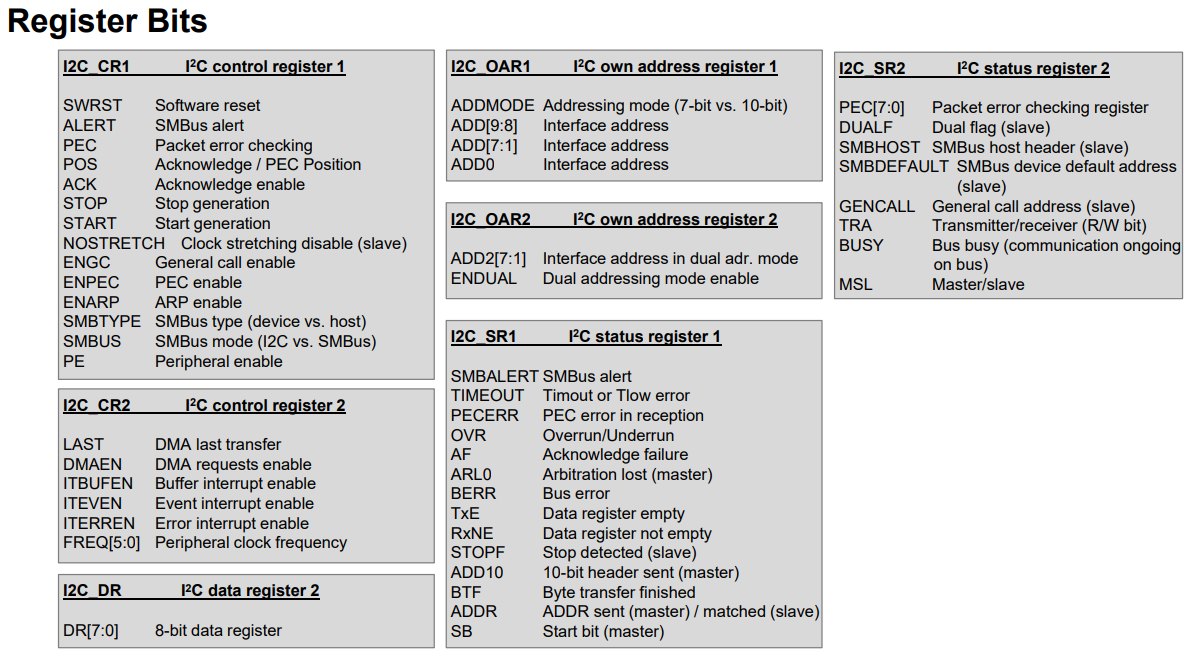
\includegraphics[width=\linewidth]{i2c_registerbits.png}









